\documentclass[11pt]{article} % use larger type; default would be 10pt

\usepackage[slovene]{babel}
\usepackage[utf8]{inputenc}
\usepackage[T1]{fontenc}

\usepackage{amsmath}
\usepackage{amsthm}
\usepackage{amsfonts}
\usepackage{url}
\usepackage{graphicx}
\usepackage{enumerate}


\renewcommand\thesection{}
\renewcommand\thesubsection{\thesection \alph{subsection})}


\begin{document}
\begin{titlepage}
	\centering
	{\scshape\LARGE Fakulteta za matematiko in fiziko \par}
	\vspace{1cm}
	{\scshape\Large Iterativne numerične metode v lienarni algebri\par}
	\vspace{1.5cm}
	{\huge\bfseries 1.domača naloga\par}
	\vspace{2cm}
	{\Large\itshape Miha Avsec\par}
	\vfill

	\vfill

% Bottom of the page
	{\large \today\par}
\end{titlepage}

Naloga je bila samostojno reševana s porgramom Matlab 2016a.

\section{1.naloga}

Prvo nalogo rešujemo s pomočjo ugrajenih funkcij numgrid in delsq. Najprej konstruiramo matriko delilnih točk, kjer so te točke v obliki plusa. To je narejeno s pomočjo funkcije numgridPlus.
Funkciji podamo število točk na katere želimo razdeliti naše območje. Število točk mora biti v obliki $k*3 +2$, saj imamo dve zunanji točki notranji del območja pa moramo enakomerno razdeliti na $3$ dele. V funkciji numgridPlus zaporedoma kličemo funkcijo numgrid('S',n+2). kjer je $n = ((k*3+2)-2)/3$. Paziti moramo da prištejemo $2$ točki saj moramo upoštevati, da numgrid('S',n+2) razdeli kvadrat na $n+2$ točk od katerih sta $2$ robni. Končni integral nato izračunamo s funkcijo integral(N,risi), kjer je $N$ število točk, ki jih podamo kot argument funkciji numgridPlus. Risi pa pove ali problem narišemo ali ne. Funkcija integral nastavi levo stran sistema s pomočjo funkcij numgridPlus in delsq. Za desno stran sistema pa vzamemo $2\cdot h^2 \cdot e_1$. Tako dobimo $U$ rešitev sistema v danem območju, da pa izračunamo integral množimo z matriko $t\cdot t'$, kjer je $t$ oblike
$$[1,2,2, \ldots, 2,1].$$
 Za boljši približek integrala na koncu interpoliramo vrednosti integrala glede na število delilnih točk in potem ta interpolant izračunamo v točki nič, ki naj bi predstavljala ničelno napako. Končni rezultat je tako $0.471081327583354$, ki ga dobimo s klicom skripte nal1.

Na spodnji sliki je prikazana slika območja, ki ga dobimo pri reševanju problema.

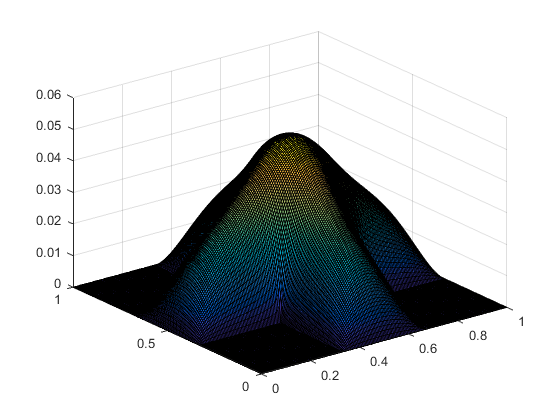
\includegraphics[width=0.6\textwidth]{slika1}

\section{2.naloga}

Naloga je rešena s funkcijo DLanczosPivot(A,b,x0,tol,maxit), ki dobi enake vhodne podatke, kot funkcija DLanczos. Funkcija deluje tako, da preveri ali bo trenutnem koraku diagonalni element $0$ ali blizu ničle. V tem primeru gre funkcija v vejo pivotiranja, v nasprotnem primeru pa se korak izvede enako, kot pri DLanczosu. Če je element blizu ničle moramo izvesti pivotiranje. Element prve poddiagonale matrike L $l(j)$ izračunamo, kot $u(j-1)/b(j-1)$, kjer je $u$ diagonala matrike $U$, ter $b$ naddiagonala matrike $T$. Novi $u(j)$ izračunamo kot,
$u(j) = b(j) -l(j)*a(j)$, kjer je a idagonala matrike $T$. Novo formula za izračun vektorja $z$ se glasi $z(j) = -l(j)*z(j-1)-l(j-1)*z(j-2)$. Novi vekotr p pa izračunamo po formuli
$p = 1/u(j)*(vz - a(j)*p-b(j)*pz)$, kjer je $vz$ novi vektor matike $V$, $pz$ pa je predzadnji vekotr matrike $P$. 


\section{3.naloga}

\subsection{Matrika c-63}

Matrika $c-63$ je simetrična, vendar ni pozitivno definitna.

 Konvergenca gmres brez predpogojevanja je počasna, saj $1000$ korakov metode zadošča le za ostanek velikosti $10^{-2}$. S predpogojevanjem pa lahko konvergenco pospešimo. Uporabimo lahko le nepopolni LU razcep saj matrika ni pozitivno definitna. A kljub predpogojevanju z delnim LU, kjer odstranimo elemente manjše od $0.1$ metoda še vedno ne skonvergira do natančnosti $10^{-6}$ po $300$ korakih. Optimalna izbira velikosti podprostora je $25$, saj je tako časovna zahtevnost kot tudi število korakov majhno.

 Podobno, kot pri gmres je tudi pri minres konvergenca pocasna. Po $1000$ korakih imamo ostanek velikosti $10^{-1}$. Pri minres si ne moremo pomagati s predpogojevanjem ker delni LU razcep ni  simetričen in pozitivno definiten.
 
 Metode pcg ne moremo uporabiti, ker matrika ni pozitivno definitna.
 
 Metoda qmr konvergira pocasi.  Po $1000$ korakih imamo ostanek velikosti $10^{-1}$. Z enakim LU razcepom kot pri gmres je za željeni ostanek metoda potrebovala dobrih 700 korakov. A je za to potrebovala skoraj dvakrat toliko časo kot gmres(25).
 
 Metoda bicg brez predpogojevanja ni delovala. S predpogojevanjem pa je metoda prišla do približka, a le ta je bil slabši kot približek metode qmr izračunan v podobnem času.
 
Metoda bicg-stab brez predpogojevanja ni prišla do rezultata. S predpogojevanjem, pa je metoda dala rezultat, a je bila konvergenca se vedno pocasna.

Metoda symmlq nam v tem primeru ni dala odgovora, predpogojevanje pa nismo mogli izvesti, saj pri LU razcepu ne dobimo simetrične pozitivne matrike.

Najbolje se je na dani matriki odrezala metoda gmres s ponovnim zagonom.

Pričakovali bi, da se bo glede na obliko matrike najbolje odrezala metoda minres, a je konvergenca prepočasna, za predpogojevanje pa ne moremo uporabiti LU ali razcepa Choleskega. Glede na obliko pa se bi morala dobro obnesti tudi metoda gmres, ki je res najbolša za to matriko. Ce hočemo imete napako velikosti $10^{-3}$ ali več, pa metoda gmres(25) deluje hitreje kakor reševanje sistema v matlabu.

\subsection{Matrika gridgena}

Konvergenca te matrike je izjemno hitra že brez predpogojevanja. Uporabimo lahko vse metode, saj je matrika simetrična in pozitivno definitna. Pričakovali bi, da se bo najbolje odrezala metoda pcg zaradi strokture matrike, a temu ni tako. Najbolje od vseh metod se je odrezala metoda bicgstab, ki je za izračun potrebovala najmanj časa. S to metodo lahko tudi za veliko natančnost $10^{10}$ sistem rešimo hitreje, kot z ugrajeno matlabovo metodo $A\textbackslash b$.

\subsection{Matrika rajat25}

Matrika $rajat25$ ni ne simetrična ne pozitivno definitna. Konvergenca je pri vseh metodah, ki jih lahko uporabimo počasna. Za predpogojevanje ne moremo uporabiti LU razcepa saj imamo na diagonali ničelne elemente, prav tako pa ne moremo uporabiti razcepa choleskega.  Na voljo imamo le metode gmres, bicg, qmr, bicgstab. Najbolje se je odrezala metoda bicgsta če smo dopustili veliko število korakov, a se napaka ni dosti izboljšala. Za večjo napako okoli $10^{-3}$ pa je najboljša metoda qmr, kar bi tudi pričakovali glede na odločitveno drevo. Če smo zadovoljni s z ostankom okoli $10^-{-3}$, potem vse metode delujejo hitreje kakor reševanje sistema.

\section{4.naloga}

S pomočjo funkcije ocena določimo optimalen $\alpha$, pri katerem želimo računati celoten inverz. Funkcija ocena za različne $\alpha$  poračuna pcg(A,b) in shrani potrebno število korakov, ostanek metode in časovno zahtevnost metode. Na koncu za vse nariše grafe v odvisnosti od $\alpha$. 

\begin{figure}[ht]
\centering
\begin{minipage}{.5\textwidth}
\centering
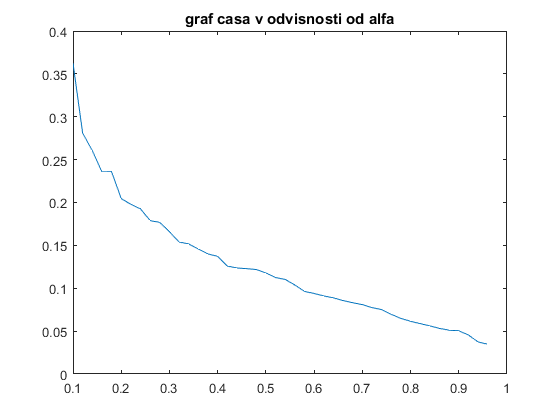
\includegraphics[scale=0.5]{cas}
%\captionof{figure}{Graf časa v odvisnosti od $\alpha$.}
%\label{fig:krivulja}
\end{minipage}%
\begin{minipage}{.5\textwidth}
\centering
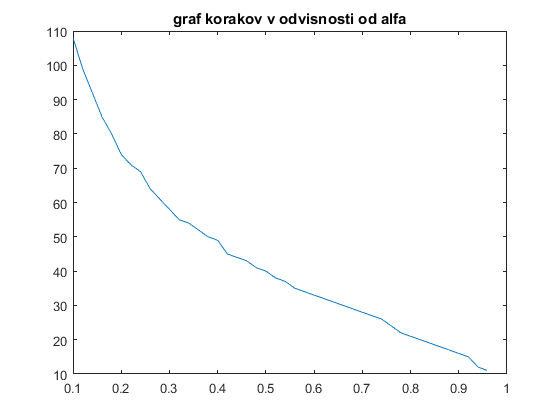
\includegraphics[scale=0.5]{koraki}
%\captionof{figure}{Graf števila korakov v odvisnosti od $\alpha$.}
%\label{projektivnaz}
\end{minipage}
\end{figure}

\begin{figure}[ht]
\centering
\begin{minipage}{.5\textwidth}
\centering
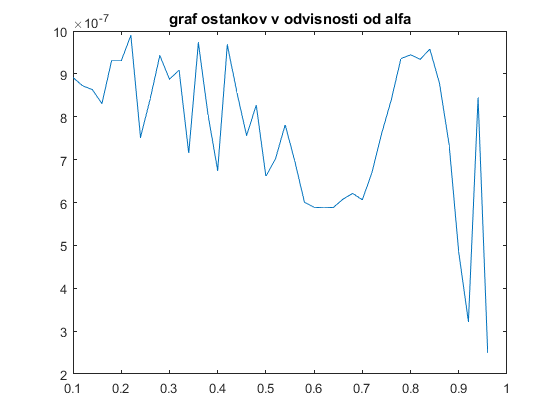
\includegraphics[scale=0.5]{ostanek}
%\captionof{figure}{Graf ostankov v odvisnosti od $\alpha$.}
%\label{fig:krivulja}
\end{minipage}%
\end{figure}


Vidimo, da se optimalen $\alpha$ nahaja okoli $0.7$, saj so ostanki dobri časovna zahtevnost pa je tam majhna. Ko izberemo $\alpha$ poženemo funkcijo RegularizacijaInverz(B,test,20489,razlika,100), kjer je B funkcija množenja matrike pri danem $\alpha$, test je matrika s katero hočemo množiti, $20489$ je velikost matrike train, razlika je zahtevana natančnost, $100$ pa je število korakov posamezne metode pcg. Funkcija deluje tako, da za vsak enotski vektor izračuna inverzni stolpec matrike B, ki ga pomnoži z test' in ga shrani v začasni matriki. V vsakem koraku izračuna še razliko
$$||train*train'*inverznispolpec(i) - e_i||_{\infty}.$$
Ostanek je potem največja od teh razlik. Končna rešitev se nahaja v datoteki $resitev.mat$.

\end{document}
